% remember to put in tool design
% interview Q's etc - mirror sections from study part 1
To better understand how students think about privacy when choosing between VPN providers, we designed a small-scale lab study.
The results of the interviews and the survey described in sections~\ref{} suggested that privacy was not of significant concern to students when choosing a VPN provider to use.
Nonetheless, we wanted to assess if students would value their privacy more if they were given more information about the privacy practices of VPN providers.
\AH{Should I add a short blurb about what kind of experiment we designed?}

\subsection{Recruitment} 
We once again recruited participants through listservs maintained by our institution's survey center.
We filtered for students who had used a VPN before, who had not participated in the interview or survey studies, and were currently undergraduate or graduate students at our institution. 
All interviews were audio-taped, and participants were compensated with a \$20 Amazon gift card.

In total, 64 people responded to our recruitment e-mails but some were ineligible as they had completed the interview or survey or were not students.
We were able to conduct our experiment with 14 of the 65 eligible participants.
However, we had to discard two interviews owing to audio related issues and since one of the participants had actually participated in the survey.
This left us with valid data from 12 participants.

\subsection{Pre-study Survey} 
Before participating in the study, respondents were asked to fill out a consent form and a short survey where we collected demographic information.
In the survey, participants confirmed that they have used a VPN before, and they listed the VPNs they have used in the past.
Participants also gave consent to audio recording for the experiment.

We also asked the participants several multiple choice questions to elicit their views on privacy with respect to VPNs.
For example, we asked participants who they think has access to their data while using a VPN.
We also asked participants what kinds of data they think are being shared.
These questions gave us a broad understanding of the views participants had about VPNs before participating in the experiment.

\subsection{Participants} 
\mc{can we summarize some of this in a table?}
According to the results of our pre-study survey, 9 of our 12 participants were between the ages of 18 and 24 (75\%) and 3 participants were between the ages of 25 and 34 (25\%).
Of these participants, 7 were females (58.3\%), and 5 were males (41.7\%).
Furthermore, 7 of the participants were from the United States (58.3\%), and 5 participants were of other nationalities (41.7\%). 
Lastly, 4 of the participants were computer science students (33.3\%), 3 of the participants were political science students (25\%), and 5 of the participants were studying other majors (41.7\%).

With respect to VPN usage, 8 participants indicated that they have used institutional VPNs (66.7\%), and 3 participants indicated that they have used VPNs that their employers offered (25\%).
Furthermore, 6 participants indicated that they have used a paid, commercial VPN (41.7\%), and 5 participants indicated that they have used a free, commercial VPN (50\%).
Interestingly, 1 participant indicated that they have used a VPN that they set up themselves (8.3\%).

Lastly, with respect to privacy, 10 participants indicated that they have not looked through a VPN provider's privacy policy (83.3\%), with only 2 participants indicating otherwise (16.7\%).
Every participant believed their VPN provider has access to their location (100\%).
Furthermore, 8 of the participants believed their VPN provider collects data about which websites they visit (66.7\%).
Interestingly, 7 of the participants believe VPNs guarantee access to the Internet (58.3\%), 6 of the participants believe VPNs mask their IP address (50\%), and 4 participants believe VPNs guarantee safety from tracking (33.3\%).
However, only 1 participant believes VPNs guarantee anonymity (8.3\%), and only 1 participant believes VPNs guarantee "privacy" (8.3\%).
 
\subsection{Laboratory Study Design}
\AH{Should we add a blurb about the overall design of the study?}

\subsubsection{VPN Audit Extension}
\begin{figure}[t]
    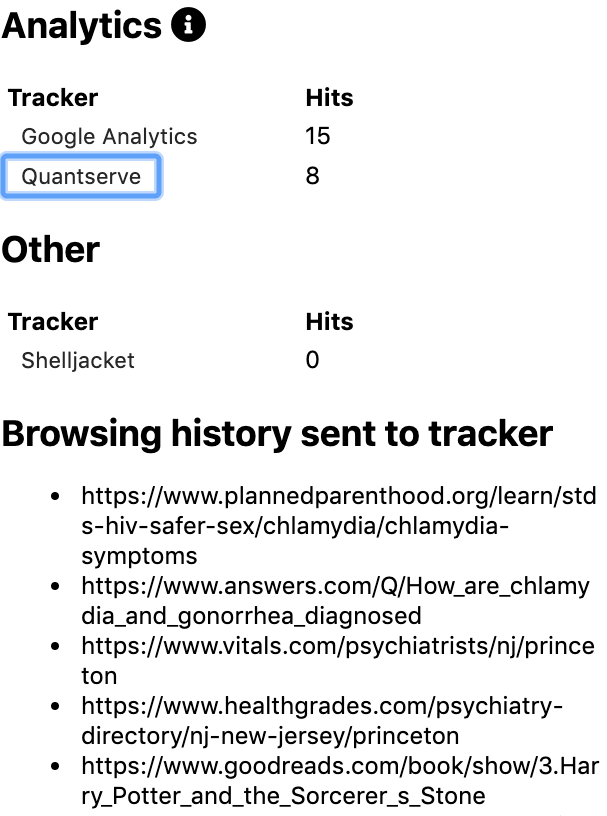
\includegraphics[width=0.85\linewidth]{sections/figures/vpn-audit.png}
    \caption{A screenshot of our Chrome extension for showing the browsing history sent to trackers outside of Hotspot Shield.}
    \label{fig:vpn-audit}
\end{figure}

Hotspot Shield--a free VPN provider--sends data to select trackers through its Chrome extension~\cite{windscribe-hotspot-shield}. \mc{isn't it also the most popular vpn, add ref to indicate as much} According to the PAC \mc{describe what this is for} file in the extension, if an object on a webpage that points to the domains "analytics.google.com" (owned by Google), "pixel.quantserve.com" (owned by Quantcast), or "shelljacket.us", then any connections to these domains are created outside of the VPN.
\AH{Should we show the code for the PAC file here as a figure?} \mc{yes, show and highlight the relevant piece with an annotation or caption}
This means Google and Quantcast can see which websites users of Hotspot Shield are visiting, even while the users are using the VPN. \mc{say why this is a data leakage per se}

We developed VPNAudit as a Chrome extension to show users the privacy leaks in HotSpotShied and design a laboratory study to see how university students would react.
Figure~\ref{fig:vpn-audit} shows a screenshot of our extension.
The extension works by examining webpages in real time that users visit while using Hotspot Shield and looking for the Google Analytics, Quantserve, and Shelljacket trackers.
It then counts the number of unique webpage that these trackers were present on.
When a user clicks on the name of a tracker, they see a list of each unique webpage under the "Browsing history sent to tracker" heading. \mc{need to explain why this is important}

\subsubsection{Interview Questions}
After the participants completed the pre-study survey, we scheduled times for each participant to conduct the experiment with a member of the research team.
Each participant again consented to audio recording and confirmed that they have used a VPN before.
We then explained to the participants that the purpose of the study was to understand how university students choose between VPN providers and what factors are most important to them, e.g. ease of use, privacy, and security.

Once we began recording audio, we asked the participants to watch a short video on the website for Hotspot Shield about how VPNs work.
We instructed them to watch this video so that each participant would have a general understanding of the claims that Hotspot Shield makes with respect to privacy.
After the video ended, we asked the participants to look around the Hotspot Shield website 
Each participant was then instructed to turn on the Hotspot Shield extension on their own and configure it to their liking.



Interview questions go here \mc{add in the tasks they were asked to complete and the protocol you followed during the interviews including showing them screenshots (did you do that?) etc}

\subsection{Analysis}
We first transcribed the recordings from each session and developed a code book to apply to the transcripts.
Our code book was based on general trends we discovered from an initial reading of the transcriptions.
The codes created related to choosing VPN providers, perceptions of privacy with respect to VPNs, and reactions to VPNAudit.
In total, we created 13 parent codes and 68 child codes. \mc{add example codes} The research team then discussed the coded transcripts and the final themes emerging from the lab sessions are discussed here.

\subsection{Limitations}
There are several limitations of our participant demographics that must be considered.
For example, our sample size was limited to 12 participants, which means that our findings cannot generalize to all university students.
Our participants are also mostly Computer Science students that may be more technically sophisticated than students of other disciplines.
Most of our participants are from the United States, which limits our ability to understand how international students think about privacy with respect to VPNs.
Lastly, all of our participants were students at a particular university.

We are also limited by our experiment design in several ways.
Our participants were only exposed to the privacy practices of Hotspot Shield, so we are unable to generalize how they would react to the privacy practices of other VPN providers.
We are also unable to gauge how participants would react to the privacy practices of VPN providers on their own computers and within their own personal space; at best, we can ask them to imagine.